% answers.tex —— 1992 年·上海卷 · 参考答案与详细解析片段
% 由 tools/generate_projects.py 依来源总账自 1992/1992_上海_试题.md + 1992/1992_上海_解析正文.md + 1992/1992_上海_答案要点.md 生成，勿手改（改源 MD 后重跑）


卷内第 1—10 题只列结果、第 11—20 题只列代号，第 21—26 题给出带分步给分的完整解答。以下按题整理，填空与选择题补出必要的推导，解答题以卷内解法为主线重述。

\gkpart{一、填空题（第 1—10 题）}

\begin{answer}
\gksolhead{1}{}

\textbf{题目}：

求值：$\cos\dfrac{5\pi}{8}\cos\dfrac{\pi}{8}=$ \gkblank{}。

\Needspace{4\baselineskip}
\textbf{解析}

\Needspace{5\baselineskip}
由 $\dfrac{5\pi}{8}=\pi-\dfrac{3\pi}{8}$ 得 $\cos\dfrac{5\pi}{8}=-\cos\dfrac{3\pi}{8}=-\sin\dfrac{\pi}{8}$。于是

\nopagebreak[4]
\[
\cos\frac{5\pi}{8}\cos\frac{\pi}{8}=-\sin\frac{\pi}{8}\cos\frac{\pi}{8}=-\frac{1}{2}\sin\frac{\pi}{4}=-\frac{\sqrt{2}}{4}.
\]

\gkanswer{答案：$-\dfrac{\sqrt{2}}{4}$。}

\end{answer}
\begin{answer}
\gksolhead{2}{}

\textbf{题目}：

$\left(x+\dfrac{1}{x}\right)^{8}$ 的展开式中 $\dfrac{1}{x^{2}}$ 的系数是 \gkblank{}（结果用数值表示）。

\Needspace{4\baselineskip}
\textbf{解析}

\Needspace{5\baselineskip}
展开式的第 $k+1$ 项为

\nopagebreak[4]
\[
T_{k+1}=C_{8}^{k}x^{8-k}\left(\frac{1}{x}\right)^{k}=C_{8}^{k}x^{8-2k}.
\]

令 $8-2k=-2$，得 $k=5$，故 $\dfrac{1}{x^{2}}$ 的系数为 $C_{8}^{5}=C_{8}^{3}=56$。

\gkanswer{答案：$56$。}

\end{answer}
\begin{answer}
\gksolhead{3}{}

\textbf{题目}：

函数 $y=\sin^{2}x-\sin x\cos x+\cos^{2}x$ 的最大值是 \gkblank{}。

\Needspace{4\baselineskip}
\textbf{解析}

\Needspace{5\baselineskip}
利用 $\sin^{2}x+\cos^{2}x=1$ 与 $2\sin x\cos x=\sin 2x$，

\nopagebreak[4]
\[
y=1-\sin x\cos x=1-\frac{1}{2}\sin 2x.
\]

当 $\sin 2x=-1$ 时 $y$ 取最大值 $1+\dfrac{1}{2}=\dfrac{3}{2}$。

\gkanswer{答案：$\dfrac{3}{2}$。}

\end{answer}
\begin{answer}
\gksolhead{4}{}

\textbf{题目}：

方程 $\log_{5}(x+1)-\log_{\frac{1}{5}}(x-3)=1$ 的解是 \gkblank{}。

\Needspace{4\baselineskip}
\textbf{解析}

\Needspace{5\baselineskip}
定义域要求 $x>3$。由换底关系

\nopagebreak[4]
\[
\log_{\frac{1}{5}}(x-3)=\frac{\log_{5}(x-3)}{\log_{5}\frac{1}{5}}=-\log_{5}(x-3),
\]

\Needspace{5\baselineskip}
原方程化为 $\log_{5}(x+1)+\log_{5}(x-3)=1$，即

\nopagebreak[4]
\[
(x+1)(x-3)=5,\qquad x^{2}-2x-8=0,
\]

解得 $x=4$ 或 $x=-2$；由 $x>3$ 舍去 $x=-2$，故 $x=4$。

\gkanswer{答案：$4$。}

\end{answer}
\begin{answer}
\gksolhead{5}{}

\textbf{题目}：

计算 $(\sqrt{3}+i)^{6}=$ \gkblank{}（$i$ 是虚数单位）。

\Needspace{4\baselineskip}
\textbf{解析}

\Needspace{5\baselineskip}
$\sqrt{3}+i=2\left(\cos\dfrac{\pi}{6}+i\sin\dfrac{\pi}{6}\right)$，由棣莫弗定理

\nopagebreak[4]
\[
(\sqrt{3}+i)^{6}=2^{6}\left(\cos\pi+i\sin\pi\right)=64\cdot(-1)=-64.
\]

\gkanswer{答案：$-64$。}

\end{answer}
\begin{answer}
\gksolhead{6}{}

\textbf{题目}：

如果直线 $l$ 与直线 $x+y-1=0$ 关于 $y$ 轴对称，那么直线 $l$ 的方程是 \gkblank{}。

\Needspace{4\baselineskip}
\textbf{解析}

\Needspace{5\baselineskip}
关于 $y$ 轴对称的变换为 $(x,y)\mapsto(-x,y)$。设 $l$ 上点为 $(x,y)$，则 $(-x,y)$ 在已知直线上，即 $-x+y-1=0$，整理得 $l$ 的方程

\nopagebreak[4]
\[
x-y+1=0.
\]

\gkanswer{答案：$x-y+1=0$。}

\end{answer}
\begin{answer}
\gksolhead{7}{}

\textbf{题目}：

已知圆台的下底面半径为 8cm，高为 6cm，母线与下底面成 $45^{\circ}$ 的角，那么圆台的侧面积是 \gkblank{} cm²（结果中保留 $\pi$）。

\Needspace{4\baselineskip}
\textbf{解析}

\Needspace{5\baselineskip}
设圆台上、下底面半径分别为 $r$、$R=8$，高 $h=6$，母线长 $l$。母线 $l$ 与下底面成 $45^{\circ}$ 角，故

\nopagebreak[4]
\[
l=\frac{h}{\sin 45^{\circ}}=6\sqrt{2},\qquad R-r=\frac{h}{\operatorname{tg}45^{\circ}}=6,
\]

\Needspace{5\baselineskip}
于是 $r=2$。侧面积

\nopagebreak[4]
\[
S_{\text{侧}}=\pi(R+r)l=\pi\cdot 10\cdot 6\sqrt{2}=60\sqrt{2}\,\pi.
\]

\gkanswer{答案：$60\sqrt{2}\,\pi$。}

\end{answer}
\begin{answer}
\gksolhead{8}{}

\textbf{题目}：

已知函数 $y=f(x)$ 的反函数是 $f^{-1}(x)=\sqrt{x}-1\ (x\ge 0)$，那么函数 $y=f(x)$ 的定义域是 \gkblank{}。

\Needspace{4\baselineskip}
\textbf{解析}

$f$ 的定义域等于其反函数 $f^{-1}$ 的值域。当 $x\ge 0$ 时 $\sqrt{x}-1\ge -1$，故 $y=f(x)$ 的定义域为 $[-1,+\infty)$。

\gkanswer{答案：$[-1,+\infty)$。}

\end{answer}
\begin{answer}
\gksolhead{9}{}

\textbf{题目}：

由 1，2，3，4，5 组成比 40000 小的没有重复数字的五位数的个数是 \gkblank{}（结果用数值表示）。

\Needspace{4\baselineskip}
\textbf{解析}

\Needspace{5\baselineskip}
五位数小于 40000，故万位数字只能取 1、2、3，共 3 种；其余四位由剩下四个数字任意排列，有 $4!=24$ 种。总数为

\nopagebreak[4]
\[
3\times 4!=72.
\]

\gkanswer{答案：$72$。}

\end{answer}
\begin{answer}
\gksolhead{10}{}

\textbf{题目}：

如图，直平行六面体 $A_{1}C$ 的上底面 $ABCD$ 为菱形，$\angle BAD=60^{\circ}$，侧面为正方形。$E$、$F$ 分别是 $A_{1}B_{1}$、$AA_{1}$ 的中点，$M$ 是 $AC$ 与 $BD$ 的交点，则 $EF$ 与 $B_{1}M$ 所成角的大小为 \gkblank{}（用反三角函数表示）。
\nopagebreak[4]
\begin{center}% 1992 年上海卷第 10 题：直平行六面体 A₁C，上底面 ABCD 为菱形，E 为 A₁B₁ 中点，F 为 AA₁ 中点，M 为 AC 与 BD 的交点
% 依固定扫描页重绘，只画拓扑与标号，不按比例
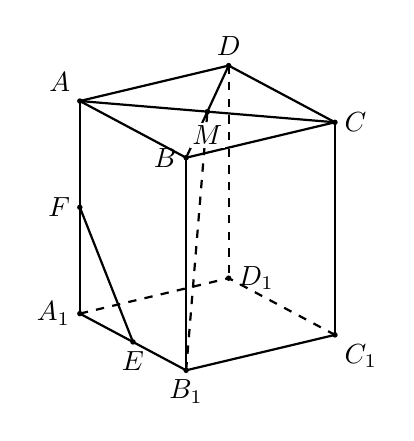
\begin{tikzpicture}[>=stealth,scale=0.9,line join=round]
  % 上底面 ABCD
  \coordinate (A) at (-2,0.9);
  \coordinate (B) at (-0.5,0.1);
  \coordinate (C) at (1.6,0.6);
  \coordinate (D) at (0.1,1.4);
  % 下底面 A1B1C1D1（向下平移）
  \coordinate (A1) at (-2,-2.1);
  \coordinate (B1) at (-0.5,-2.9);
  \coordinate (C1) at (1.6,-2.4);
  \coordinate (D1) at (0.1,-1.6);
  \coordinate (M) at (-0.2,0.75);
  \coordinate (E) at (-1.25,-2.5);
  \coordinate (F) at (-2,-0.6);

  % 可见棱
  \draw[thick] (A)--(B)--(C)--(D)--cycle;
  \draw[thick] (A)--(A1);
  \draw[thick] (B)--(B1);
  \draw[thick] (C)--(C1);
  \draw[thick] (A1)--(B1)--(C1);
  % 不可见棱
  \draw[thick,dashed] (A1)--(D1)--(C1);
  \draw[thick,dashed] (D)--(D1);
  % 上底面对角线 AC、BD 与交点 M
  \draw[thick] (A)--(C);
  \draw[thick] (B)--(D);
  % EF
  \draw[thick] (E)--(F);
  \draw[thick,dashed] (B1)--(M);

  \fill (A) circle (1.1pt) node[above left] {$A$};
  \fill (B) circle (1.1pt) node[left] {$B$};
  \fill (C) circle (1.1pt) node[right] {$C$};
  \fill (D) circle (1.1pt) node[above] {$D$};
  \fill (A1) circle (1.1pt) node[left] {$A_{1}$};
  \fill (B1) circle (1.1pt) node[below] {$B_{1}$};
  \fill (C1) circle (1.1pt) node[below right] {$C_{1}$};
  \fill (D1) circle (1.1pt) node[right] {$D_{1}$};
  \fill (M) circle (1.1pt) node[fill=white,inner sep=1pt,below=4pt] {$M$};
  \fill (E) circle (1.1pt) node[below] {$E$};
  \fill (F) circle (1.1pt) node[left] {$F$};
\end{tikzpicture}
\end{center}
\nopagebreak[4]
（源疑点：立体名称卷面印作「直平行六面体 $A_{1}C$」；按图形与「上底面 $ABCD$」的标注惯例，通常应记作 $AC_{1}$。照录卷面，未改。）

\Needspace{4\baselineskip}
\textbf{解析}

\Needspace{5\baselineskip}
设棱长为 $a$。取下底面 $A_{1}B_{1}C_{1}D_{1}$ 所在平面为 $z=0$，上底面 $ABCD$ 在平面 $z=a$ 内。由 $\angle BAD=60^{\circ}$ 及菱形边长为 $a$，取

\nopagebreak[4]
\[
A(0,0,a),\quad B(a,0,a),\quad D\left(\frac{a}{2},\frac{\sqrt{3}a}{2},a\right),\quad C\left(\frac{3a}{2},\frac{\sqrt{3}a}{2},a\right),
\]

\Needspace{5\baselineskip}
对应地下底面顶点为 $A_{1}(0,0,0)$、$B_{1}(a,0,0)$。于是

\nopagebreak[4]
\[
E\left(\frac{a}{2},0,0\right),\qquad F\left(0,0,\frac{a}{2}\right),\qquad M\left(\frac{3a}{4},\frac{\sqrt{3}a}{4},a\right).
\]

\Needspace{5\baselineskip}
从而

\nopagebreak[4]
\[
\overrightarrow{EF}=\left(-\frac{a}{2},0,\frac{a}{2}\right),\qquad
\overrightarrow{B_{1}M}=\left(-\frac{a}{4},\frac{\sqrt{3}a}{4},a\right).
\]

\Needspace{5\baselineskip}
计算得

\nopagebreak[4]
\[
|\overrightarrow{EF}|=\frac{a}{\sqrt{2}},\qquad |\overrightarrow{B_{1}M}|=\frac{\sqrt{5}}{2}a,\qquad
\overrightarrow{EF}\cdot\overrightarrow{B_{1}M}=\frac{5a^{2}}{8}.
\]

\Needspace{5\baselineskip}
故两向量夹角的余弦为

\nopagebreak[4]
\[
\frac{\frac{5a^{2}}{8}}{\frac{a}{\sqrt{2}}\cdot\frac{\sqrt{5}a}{2}}=\frac{\sqrt{10}}{4}.
\]

两直线所成角取锐角，其余弦为 $\dfrac{\sqrt{10}}{4}$，正弦为 $\sqrt{1-\dfrac{10}{16}}=\dfrac{\sqrt{6}}{4}$，故所成角为 $\arcsin\dfrac{\sqrt{6}}{4}$。

\gkanswer{答案：$\arcsin\dfrac{\sqrt{6}}{4}$。}

\end{answer}
\gkpart{二、选择题（第 11—20 题）}

\begin{answer}
\gksolhead{11}{}

\textbf{题目}：

当 $0<a<1$ 时，函数 $y=a^{x}$ 和 $y=(a-1)x^{2}$ 的图象只可能是（　）。
\nopagebreak[4]
\begin{center}% 1992 年上海卷第 11 题：四个函数图象选项（A）～（D）
% 每图均为 y=a^x 与 y=(a-1)x^2 的搭配；依固定扫描页重绘，只画拓扑与标号，不按比例
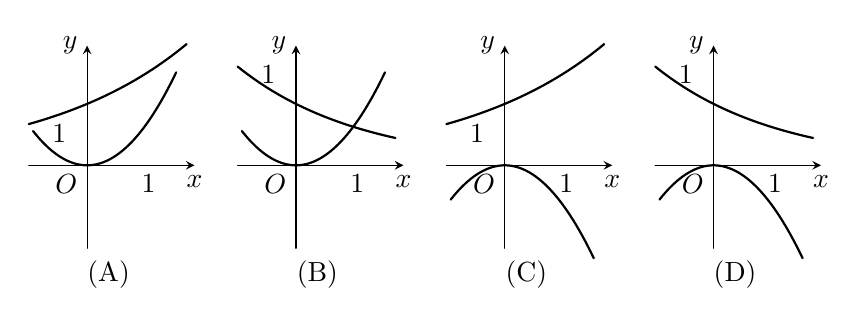
\begin{tikzpicture}[>=stealth,scale=0.78,line cap=round]
  % (A) 指数递增 + 抛物线开口向上
  \begin{scope}
    \draw[->] (-0.95,0)--(1.75,0) node[below] {$x$};
    \draw[->] (0,-1.35)--(0,1.95) node[left] {$y$};
    \node[below left] at (0,0) {$O$};
    \node[below] at (1,0) {$1$};
    \node[below left=4pt] at (0,1) {$1$};
    \draw[thick,domain=-0.95:1.62,samples=60] plot (\x,{exp(0.42*\x)});
    \draw[thick,domain=-0.88:1.45,samples=50] plot (\x,{0.72*\x*\x});
    \node at (0.35,-1.78) {(A)};
  \end{scope}
  % (B) 指数递减 + 抛物线开口向上
  \begin{scope}[xshift=3.4cm]
    \draw[->] (-0.95,0)--(1.75,0) node[below] {$x$};
    \draw[->] (0,-1.35)--(0,1.95) node[left] {$y$};
    \node[below left] at (0,0) {$O$};
    \node[below] at (1,0) {$1$};
    \node[above left=4pt] at (0,1) {$1$};
    \draw[thick,domain=-0.95:1.62,samples=60] plot (\x,{exp(-0.50*\x)});
    \draw[thick,domain=-0.88:1.45,samples=50] plot (\x,{0.72*\x*\x});
    \node at (0.35,-1.78) {(B)};
  \end{scope}
  % (C) 指数递增 + 抛物线开口向下
  \begin{scope}[xshift=6.8cm]
    \draw[->] (-0.95,0)--(1.75,0) node[below] {$x$};
    \draw[->] (0,-1.35)--(0,1.95) node[left] {$y$};
    \node[below left] at (0,0) {$O$};
    \node[below] at (1,0) {$1$};
    \node[below left=4pt] at (0,1) {$1$};
    \draw[thick,domain=-0.95:1.62,samples=60] plot (\x,{exp(0.42*\x)});
    \draw[thick,domain=-0.88:1.45,samples=50] plot (\x,{-0.72*\x*\x});
    \node at (0.35,-1.78) {(C)};
  \end{scope}
  % (D) 指数递减 + 抛物线开口向下
  \begin{scope}[xshift=10.2cm]
    \draw[->] (-0.95,0)--(1.75,0) node[below] {$x$};
    \draw[->] (0,-1.35)--(0,1.95) node[left] {$y$};
    \node[below left] at (0,0) {$O$};
    \node[below] at (1,0) {$1$};
    \node[above left=4pt] at (0,1) {$1$};
    \draw[thick,domain=-0.95:1.62,samples=60] plot (\x,{exp(-0.50*\x)});
    \draw[thick,domain=-0.88:1.45,samples=50] plot (\x,{-0.72*\x*\x});
    \node at (0.35,-1.78) {(D)};
  \end{scope}
\end{tikzpicture}
\end{center}
\nopagebreak[4]
\Needspace{4\baselineskip}
\textbf{解析}

由 $0<a<1$ 知 $y=a^{x}$ 单调递减，且过点 $(0,1)$；又 $a-1<0$，故 $y=(a-1)x^{2}$ 的图象是顶点在原点、开口向下的抛物线。四个选项中只有（D）同时具备这两个特征。

\gkanswer{答案：D。}

\end{answer}
\begin{answer}
\gksolhead{12}{}

\textbf{题目}：

下列函数中，在区间 $(0,1]$ 上为减函数的是（　）。

（A）$y=\log_{2}x$；（B）$y=x^{\frac{1}{8}}$；（C）$y=\cos x$；（D）$y=\arcsin x$。

（源疑点：选项（B）的指数为叠印小分数，经与同卷第 2 题上标 $x^8$ 同型比对，分母为 $8$；照录。）

\Needspace{4\baselineskip}
\textbf{解析}

在 $(0,1]$ 上：$y=\log_{2}x$ 递增；$y=x^{\frac{1}{8}}$ 递增；$y=\cos x$ 递减；$y=\arcsin x$ 递增。故选（C）。

\gkanswer{答案：C。}

\end{answer}
\begin{answer}
\gksolhead{13}{}

\textbf{题目}：

$\alpha$、$\beta$ 是两个不重合的平面，在下列条件中，可判定平面 $\alpha$ 与 $\beta$ 平行的是（　）。

（A）$\alpha$、$\beta$ 都垂直平面 $\gamma$；

（B）$\alpha$ 内不共线的三点到 $\beta$ 的距离都相等；

（C）$l$、$m$ 是 $\alpha$ 内两条直线，且 $l\parallel\beta$，$m\parallel\beta$；

（D）$l$、$m$ 是两条异面直线，且 $l\parallel\alpha$，$m\parallel\alpha$，$l\parallel\beta$，$m\parallel\beta$。

\Needspace{4\baselineskip}
\textbf{解析}

（A）两个平面都垂直同一平面时仍可相交，如坐标平面 $x=0$ 与 $y=0$ 都垂直于 $z=0$，故不能判定。

（B）取 $\beta$ 为平面 $z=0$，$\alpha$ 为平面 $x=0$，二者交于 $y$ 轴。在 $\alpha$ 内取 $A(0,0,2)$、$B(0,1,2)$、$C(0,2,-2)$，三点不共线，到 $\beta$ 的距离均为 $2$，但 $\alpha$ 与 $\beta$ 相交，故不能判定。

（C）取 $\beta$ 为平面 $z=0$，$\alpha$ 为平面 $z=x$，二者交于 $y$ 轴。在 $\alpha$ 内取两条平行直线 $l:\ (1,t,1)$、$m:\ (2,t,2)$（$t\in R$），它们的方向均为 $y$ 轴方向，与 $\beta$ 无公共点，即 $l\parallel\beta$、$m\parallel\beta$，但 $\alpha$ 与 $\beta$ 相交，故不能判定。

（D）若 $\alpha$ 与 $\beta$ 相交于直线 $c$，由 $l\parallel\alpha$ 且 $l\parallel\beta$ 可得 $l\parallel c$；同理 $m\parallel c$，于是 $l\parallel m$，与 $l$、$m$ 异面矛盾。故 $\alpha\parallel\beta$，选（D）。

\gkanswer{答案：D。}

\end{answer}
\begin{answer}
\gksolhead{14}{}

\textbf{题目}：

下列函数中，最小正周期为 $\pi$ 的偶函数是（　）。

（A）$y=\sin 2x$；（B）$y=\cos\dfrac{x}{2}$；

（C）$y=\sin 2x+\cos 2x$；（D）$y=\dfrac{1-\operatorname{tg}^{2}x}{1+\operatorname{tg}^{2}x}$。

\Needspace{4\baselineskip}
\textbf{解析}

\Needspace{5\baselineskip}
（A）$y=\sin 2x$ 是奇函数；（B）$y=\cos\dfrac{x}{2}$ 的周期为 $4\pi$；（C）$y=\sin 2x+\cos 2x=\sqrt{2}\sin\left(2x+\dfrac{\pi}{4}\right)$ 周期为 $\pi$ 但非偶函数；（D）

\nopagebreak[4]
\[
y=\frac{1-\operatorname{tg}^{2}x}{1+\operatorname{tg}^{2}x}=\cos 2x,
\]

是周期为 $\pi$ 的偶函数。选（D）。

\gkanswer{答案：D。}

\end{answer}
\begin{answer}
\gksolhead{15}{}

\textbf{题目}：

在方程 $\begin{cases}x=\sin\theta,\\ y=\cos 2\theta\end{cases}$（$\theta$ 为参数）所表示的曲线上的一点的坐标是（　）。

（A）$(2,-7)$；（B）$\left(\dfrac{1}{3},\dfrac{2}{3}\right)$；

（C）$\left(\dfrac{1}{2},\dfrac{1}{2}\right)$；（D）$(1,0)$。

\Needspace{4\baselineskip}
\textbf{解析}

消去参数：$y=\cos 2\theta=1-2\sin^{2}\theta=1-2x^{2}$，其中 $x=\sin\theta\in[-1,1]$。逐项检验：（A）$x=2$ 超出范围；（B）$1-2\cdot\dfrac{1}{9}=\dfrac{7}{9}\ne\dfrac{2}{3}$；（C）$1-2\cdot\dfrac{1}{4}=\dfrac{1}{2}$，符合；（D）$1-2=-1\ne 0$。选（C）。

\gkanswer{答案：C。}

\end{answer}
\begin{answer}
\gksolhead{16}{}

\textbf{题目}：

抛物线 $(y+2)^{2}=4(x+1)$ 的焦点坐标是（　）。

（A）$(0,-2)$；（B）$(2,2)$；

（C）$(1,-2)$；（D）$(3,2)$。

\Needspace{4\baselineskip}
\textbf{解析}

$(y+2)^{2}=4(x+1)$ 的顶点为 $(-1,-2)$，对称轴为 $y=-2$，$4p=4$ 即 $p=1$，开口向右，焦点为 $(-1+1,-2)=(0,-2)$。选（A）。

\gkanswer{答案：A。}

\end{answer}
\begin{answer}
\gksolhead{17}{}

\textbf{题目}：

下列命题中的真命题是（　）。

（A）各侧面都是矩形的棱柱是长方体；

（B）有两个相邻侧面是矩形的棱柱是直棱柱；

（C）各侧面都是等腰三角形的四棱锥是正四棱锥；

（D）有两个面互相平行，其余四个面都是等腰梯形的六面体是四棱台。

\Needspace{4\baselineskip}
\textbf{解析}

（A）各侧面都是矩形的棱柱只保证侧棱垂直于底面，底面可以不是矩形，故不一定是长方体，假。

（B）两个相邻侧面都是矩形，说明侧棱垂直于底面上两条相交直线，从而侧棱垂直于底面，棱柱为直棱柱，真。

（C）各侧面都是等腰三角形的四棱锥，其底面可以不是正方形，故不一定是正四棱锥，假。

（D）有两个面平行、其余四个面都是等腰梯形的六面体，侧棱延长后不一定交于一点，故不一定是四棱台，假。

选（B）。

\gkanswer{答案：B。}

\end{answer}
\begin{answer}
\gksolhead{18}{}

\textbf{题目}：

函数 $y=\arccos\dfrac{1}{\sqrt{x}}$ 的值域是（　）。

（A）$\left[0,\dfrac{\pi}{2}\right)$；（B）$\left(0,\dfrac{\pi}{2}\right]$；

（C）$[0,\pi)$；（D）$(0,\pi]$。

\Needspace{4\baselineskip}
\textbf{解析}

定义域为 $x\ge 1$。此时 $\dfrac{1}{\sqrt{x}}>0$，且当 $x\to+\infty$ 时 $\dfrac{1}{\sqrt{x}}\to 0^{+}$。由 $\arccos t$ 在 $(0,1]$ 上取值 $[0,\dfrac{\pi}{2})$，故值域为 $\left[0,\dfrac{\pi}{2}\right)$。选（A）。

\gkanswer{答案：A。}

\end{answer}
\begin{answer}
\gksolhead{19}{}

\textbf{题目}：

在极坐标系中，与圆 $\rho=4\sin\theta$ 相切的一条直线的方程是（　）。

（A）$\rho\sin\theta=2$；（B）$\rho\cos\theta=2$；

（C）$\rho\cos\theta=4$；（D）$\rho\cos\theta=-4$。

\Needspace{4\baselineskip}
\textbf{解析}

\Needspace{5\baselineskip}
$\rho=4\sin\theta$ 两边乘 $\rho$ 得 $\rho^{2}=4\rho\sin\theta$，即 $x^{2}+y^{2}=4y$，亦即

\nopagebreak[4]
\[
x^{2}+(y-2)^{2}=4,
\]

圆心 $(0,2)$、半径 $2$。与其相切的直线有 $y=0$、$y=4$、$x=2$、$x=-2$，即 $\rho\sin\theta=0$、$\rho\sin\theta=4$、$\rho\cos\theta=2$、$\rho\cos\theta=-2$。选项中只有 $\rho\cos\theta=2$ 是切线。选（B）。

\gkanswer{答案：B。}

\end{answer}
\begin{answer}
\gksolhead{20}{}

\textbf{题目}：

设集合 $M=\{x\mid x>2\}$，$P=\{x\mid x<3\}$，那么「$x\in M$ 或 $x\in P$」是「$x\in M\cap P$」的（　）。

（A）充分条件但非必要条件；

（B）必要条件但非充分条件；

（C）充分必要条件；

（D）非充分条件也非必要条件。

\Needspace{4\baselineskip}
\textbf{解析}

$M=\{x\mid x>2\}$，$P=\{x\mid x<3\}$，故 $M\cup P=R$，$M\cap P=(2,3)$。「$x\in M$ 或 $x\in P$」对任意实数恒成立，交集 $M\cap P$ 中的元素必属于并集 $M\cup P$，故该条件是必要条件；但并集条件不能保证 $x\in M\cap P$（如 $x=0$），故非充分。选（B）。

\gkanswer{答案：B。}

\end{answer}
\gkpart{三、解答题（第 21—23 题）}

\begin{answer}
\gksolhead{21}{}

\textbf{题目}：

（本题满分 12 分）

已知 $\cos 2\alpha=\dfrac{7}{25}$，$\alpha\in\left(0,\dfrac{\pi}{2}\right)$，$\sin\beta=-\dfrac{5}{13}$，$\beta\in\left(\pi,\dfrac{3\pi}{2}\right)$，求 $\alpha+\beta$（用反三角函数表示）。

\Needspace{4\baselineskip}
\textbf{解析}

\Needspace{5\baselineskip}
由 $\cos 2\alpha=\dfrac{7}{25}>0$ 及 $\alpha\in\left(0,\dfrac{\pi}{2}\right)$ 得 $2\alpha\in\left(0,\dfrac{\pi}{2}\right)$，故 $\alpha\in\left(0,\dfrac{\pi}{4}\right)$，且

\nopagebreak[4]
\[
\cos\alpha=\sqrt{\frac{1+\cos 2\alpha}{2}}=\sqrt{\frac{1+\frac{7}{25}}{2}}=\frac{4}{5},\qquad
\sin\alpha=\sqrt{1-\cos^{2}\alpha}=\frac{3}{5}.
\]

\Needspace{5\baselineskip}
由 $\beta\in\left(\pi,\dfrac{3\pi}{2}\right)$ 知 $\cos\beta<0$，故

\nopagebreak[4]
\[
\cos\beta=-\sqrt{1-\sin^{2}\beta}=-\sqrt{1-\frac{25}{169}}=-\frac{12}{13}.
\]

\Needspace{5\baselineskip}
于是

\nopagebreak[4]
\[
\cos(\alpha+\beta)=\cos\alpha\cos\beta-\sin\alpha\sin\beta
=\frac{4}{5}\cdot\left(-\frac{12}{13}\right)-\frac{3}{5}\cdot\left(-\frac{5}{13}\right)
=-\frac{33}{65}.
\]

\Needspace{5\baselineskip}
由 $\alpha\in\left(0,\dfrac{\pi}{4}\right)$、$\beta\in\left(\pi,\dfrac{3\pi}{2}\right)$ 得 $\alpha+\beta\in\left(\pi,\dfrac{7\pi}{4}\right)$；又 $\cos(\alpha+\beta)<0$，故 $\alpha+\beta\in\left(\pi,\dfrac{3\pi}{2}\right)$，从而

\nopagebreak[4]
\[
\alpha+\beta=\pi+\arccos\frac{33}{65}.
\]

\gkanswer{答案：$\alpha+\beta=\pi+\arccos\dfrac{33}{65}$。}

\end{answer}
\begin{answer}
\gksolhead{22}{}

\textbf{题目}：

（本题满分 12 分）

设 $w=z+ai$，其中 $a$ 是实数，$i$ 是虚数单位，$z=\dfrac{(1-4i)(1+i)+2+4i}{3+4i}$，且 $|w|\le\sqrt{2}$，求 $w$ 的辐角主值 $\theta$ 的取值范围。

\Needspace{4\baselineskip}
\textbf{解析}

\Needspace{5\baselineskip}
先化简 $z$：

\nopagebreak[4]
\[
(1-4i)(1+i)=1+i-4i-4i^{2}=5-3i,
\]

\Needspace{5\baselineskip}
故分子为 $(5-3i)+(2+4i)=7+i$，于是

\nopagebreak[4]
\[
z=\frac{7+i}{3+4i}=\frac{(7+i)(3-4i)}{25}=\frac{21-28i+3i+4}{25}=\frac{25-25i}{25}=1-i.
\]

\Needspace{5\baselineskip}
因此

\nopagebreak[4]
\[
w=z+ai=1+(a-1)i,\qquad |w|^{2}=1+(a-1)^{2}\le 2,
\]

解得 $(a-1)^{2}\le 1$，即 $0\le a\le 2$，从而 $-1\le a-1\le 1$。

\Needspace{5\baselineskip}
$w$ 的实部为 $1>0$，按卷内 $[0,2\pi)$ 口径，$\theta\in\left[0,\dfrac{\pi}{2}\right)\cup\left(\dfrac{3\pi}{2},2\pi\right)$，且 $\operatorname{tg}\theta=a-1$。由 $-1\le\operatorname{tg}\theta\le 1$ 得

\nopagebreak[4]
\[
\theta\in\left[0,\frac{\pi}{4}\right]\cup\left[\frac{7\pi}{4},2\pi\right).
\]

\gkanswer{答案：$\theta\in\left[0,\dfrac{\pi}{4}\right]\cup\left[\dfrac{7\pi}{4},2\pi\right)$。}

\end{answer}
\begin{answer}
\gksolhead{23}{}

\textbf{题目}：

（本题满分 12 分）

设动直线 $l$ 垂直于 $x$ 轴，且与椭圆 $\dfrac{x^{2}}{4}+\dfrac{y^{2}}{2}=1$ 交于 $A$、$B$ 两点，$P$ 是 $l$ 上满足 $|PA|\cdot|PB|=1$ 的点，求点 $P$ 的轨迹方程，并说明轨迹是什么图形。

\Needspace{4\baselineskip}
\textbf{解析}

\Needspace{5\baselineskip}
设 $P(x,y)$。因 $l\perp x$ 轴，$l$ 上点的横坐标均为 $x$；设 $A(x,y_{1})$、$B(x,-y_{1})$，其中 $y_{1}>0$ 且

\nopagebreak[4]
\[
\frac{x^{2}}{4}+\frac{y_{1}^{2}}{2}=1 \quad\Longrightarrow\quad y_{1}^{2}=2-\frac{x^{2}}{2},
\]

并由 $y_{1}^{2}>0$ 得 $-2<x<2$。

\Needspace{5\baselineskip}
由 $P$ 在 $l$ 上得 $|PA|=|y_{1}-y|$、$|PB|=|y_{1}+y|$，故

\nopagebreak[4]
\[
|PA|\cdot|PB|=|y_{1}^{2}-y^{2}|=1,
\]

即 $y_{1}^{2}-y^{2}=\pm 1$。代入 $y_{1}^{2}=2-\dfrac{x^{2}}{2}$：

\Needspace{5\baselineskip}
当 $y_{1}^{2}-y^{2}=1$ 时，

\nopagebreak[4]
\[
2-\frac{x^{2}}{2}-y^{2}=1 \quad\Longrightarrow\quad \frac{x^{2}}{2}+y^{2}=1;
\]

\Needspace{5\baselineskip}
当 $y_{1}^{2}-y^{2}=-1$ 时，

\nopagebreak[4]
\[
2-\frac{x^{2}}{2}-y^{2}=-1 \quad\Longrightarrow\quad \frac{x^{2}}{6}+\frac{y^{2}}{3}=1.
\]

前一椭圆满足 $|x|\le\sqrt{2}<2$，限制自然成立；后一椭圆须保留 $-2<x<2$ 的部分。

故所求轨迹为椭圆 $\dfrac{x^{2}}{2}+y^{2}=1$，以及椭圆 $\dfrac{x^{2}}{6}+\dfrac{y^{2}}{3}=1$ 夹在直线 $x=2$、$x=-2$ 之间的部分。

\gkanswer{答案：轨迹为椭圆 $\dfrac{x^{2}}{2}+y^{2}=1$，以及椭圆 $\dfrac{x^{2}}{6}+\dfrac{y^{2}}{3}=1$ 夹在直线 $x=2$、$x=-2$ 之间的部分。}

\end{answer}
\gkpart{四、解答题（第 24—26 题）}

\begin{answer}
\gksolhead{24}{}

\textbf{题目}：

（本题满分 16 分）本题共有 3 个小题，第 1 小题满分 6 分，第 2 小题满分 4 分，第 3 小题满分 6 分。

如图，圆锥的轴截面为等腰直角三角形 $SAB$，$Q$ 为底面圆周上一点。

（1）如果 $QB$ 的中点为 $C$，$OH\perp SC$，求证 $OH\perp$ 平面 $SBQ$；

（2）如果 $\angle AOQ=60^{\circ}$，$QB=2\sqrt{3}$，求此圆锥的体积；

（3）如果二面角 $A\text{-}SB\text{-}Q$ 的大小为 $\operatorname{arctg}\dfrac{\sqrt{6}}{3}$，求 $\angle AOQ$ 的大小。
\nopagebreak[4]
\begin{center}% 1992 年上海卷第 24 题：圆锥的轴截面为等腰直角三角形 SAB，Q 为底面圆周上一点
% 左图用于第 1、2 小题（含 C、H），右图用于第 3 小题
% 依固定扫描页重绘，只画拓扑与标号，不按比例
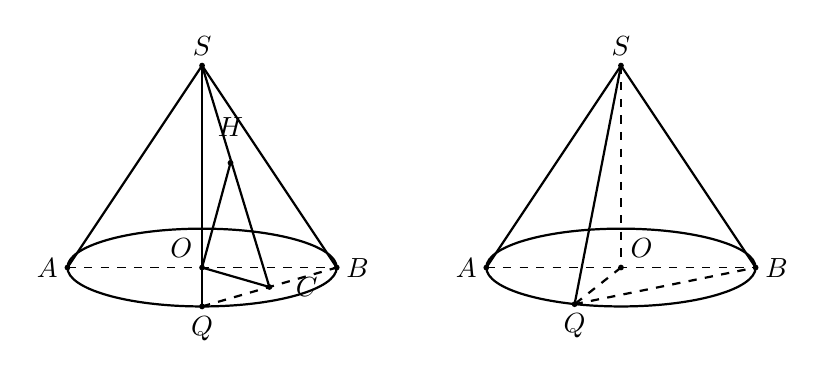
\begin{tikzpicture}[>=stealth,scale=0.95,line join=round]
  % ===== 左图 =====
  \coordinate (S)  at (0,2.7);
  \coordinate (O)  at (0,0);
  \coordinate (A)  at (-1.8,0);
  \coordinate (B)  at (1.8,0);
  \coordinate (Q)  at (0,-0.52);
  \coordinate (C)  at (0.9,-0.26);
  \coordinate (H)  at (0.38,1.40);

  \draw[thick] (0,0) ellipse (1.8 and 0.52);
  \draw[dashed] (A)--(B);
  \draw[thick] (S)--(A);
  \draw[thick] (S)--(B);
  \draw[thick,dashed] (S)--(O);
  \draw[thick,dashed] (O)--(Q);
  \draw[thick,dashed] (Q)--(B);
  \draw[thick] (S)--(Q);
  \draw[thick] (S)--(C);
  \draw[thick] (O)--(C);
  \draw[thick] (O)--(H);

  \fill (S) circle (1.1pt) node[above] {$S$};
  \fill (O) circle (1.1pt) node[above left] {$O$};
  \fill (A) circle (1.1pt) node[left] {$A$};
  \fill (B) circle (1.1pt) node[right] {$B$};
  \fill (Q) circle (1.1pt) node[below] {$Q$};
  \fill (C) circle (1.1pt) node[right=6pt] {$C$};
  \fill (H) circle (1.1pt) node[above=6pt] {$H$};

  % ===== 右图 =====
  \begin{scope}[xshift=5.6cm]
    \coordinate (S2) at (0,2.7);
    \coordinate (O2) at (0,0);
    \coordinate (A2) at (-1.8,0);
    \coordinate (B2) at (1.8,0);
    \coordinate (Q2) at (-0.62,-0.49);

    \draw[thick] (0,0) ellipse (1.8 and 0.52);
  \draw[dashed] (A2)--(B2);
    \draw[thick] (S2)--(A2);
    \draw[thick] (S2)--(B2);
    \draw[thick] (S2)--(Q2);
    \draw[thick,dashed] (S2)--(O2);
    \draw[thick,dashed] (O2)--(Q2);
    \draw[thick,dashed] (Q2)--(B2);

    \fill (S2) circle (1.1pt) node[above] {$S$};
    \fill (O2) circle (1.1pt) node[above right] {$O$};
    \fill (A2) circle (1.1pt) node[left] {$A$};
    \fill (B2) circle (1.1pt) node[right] {$B$};
    \fill (Q2) circle (1.1pt) node[below] {$Q$};
  \end{scope}
\end{tikzpicture}
\end{center}
\nopagebreak[4]
（源疑点：题面未定义 $O$、$H$；依图形与卷内解答，$O$ 为底面圆心、$H$ 为 $SC$ 上一点。照录卷面，未补写。）

\Needspace{4\baselineskip}
\textbf{解析}

（1）在 $\triangle SQB$ 中，$SQ=SB$（同一圆锥的母线长相等），$C$ 为 $QB$ 的中点，故 $SC\perp QB$。又 $OQ=OB$（底面半径），$C$ 为 $QB$ 的中点，故 $OC\perp QB$。

于是 $QB$ 垂直于平面 $SOC$ 内两条相交直线 $SC$、$OC$，即 $QB\perp$ 平面 $SOC$。因 $OH\subset$ 平面 $SOC$，得 $QB\perp OH$。

又已知 $OH\perp SC$，而 $QB$ 与 $SC$ 是平面 $SBQ$ 内两条相交直线，故 $OH\perp$ 平面 $SBQ$。

（2）$AB$ 为底面直径，$Q$ 在底面圆周上，故 $AQ\perp QB$。

\Needspace{5\baselineskip}
由 $\angle AOQ=60^{\circ}$ 知圆周角 $\angle ABQ=\dfrac{1}{2}\angle AOQ=30^{\circ}$。在 $\mathrm{Rt}\triangle AQB$ 中，

\nopagebreak[4]
\[
AB=\frac{QB}{\cos 30^{\circ}}=\frac{2\sqrt{3}}{\frac{\sqrt{3}}{2}}=4,
\]

\Needspace{5\baselineskip}
故底面半径 $OA=2$。轴截面 $SAB$ 为等腰直角三角形，$AB$ 为斜边，故高

\nopagebreak[4]
\[
SO=\frac{1}{2}AB=2.
\]

\Needspace{5\baselineskip}
圆锥体积

\nopagebreak[4]
\[
V=\frac{1}{3}\pi\cdot OA^{2}\cdot SO=\frac{1}{3}\pi\cdot 4\cdot 2=\frac{8}{3}\pi.
\]

（3）过 $Q$ 作 $QM\perp AB$，垂足为 $M$。因平面 $SAB\perp$ 底面 $ABQ$，故 $QM\perp$ 平面 $SAB$。

\Needspace{5\baselineskip}
过 $M$ 作 $MP\perp SB$，垂足为 $P$，连 $PQ$。由三垂线定理，$QP\perp SB$，故 $\angle MPQ$ 是二面角 $A\text{-}SB\text{-}Q$ 的平面角，且

\nopagebreak[4]
\[
\angle MPQ=\operatorname{arctg}\frac{\sqrt{6}}{3}.
\]

\Needspace{5\baselineskip}
设底面半径为 $R$，$\angle AOQ=\alpha$。在 $\mathrm{Rt}\triangle OMQ$ 中，

\nopagebreak[4]
\[
QM=R\sin\alpha,\qquad OM=R\cos\alpha.
\]

\Needspace{5\baselineskip}
在 $\mathrm{Rt}\triangle MPB$ 中，$\angle PBM=45^{\circ}$，$MB=OM+OB=R(1+\cos\alpha)$，故

\nopagebreak[4]
\[
MP=MB\sin 45^{\circ}=\frac{\sqrt{2}}{2}R(1+\cos\alpha).
\]

\Needspace{5\baselineskip}
于是

\nopagebreak[4]
\[
\operatorname{tg}\angle MPQ=\frac{QM}{MP}=\frac{\sqrt{2}\sin\alpha}{1+\cos\alpha}.
\]

\Needspace{5\baselineskip}
由 $\operatorname{tg}\angle MPQ=\dfrac{\sqrt{6}}{3}$ 得

\nopagebreak[4]
\[
\frac{\sin\alpha}{1+\cos\alpha}=\frac{\sqrt{3}}{3},
\]

即 $\operatorname{tg}\dfrac{\alpha}{2}=\dfrac{\sqrt{3}}{3}$，故 $\dfrac{\alpha}{2}=30^{\circ}$，$\angle AOQ=\alpha=60^{\circ}$。

\gkanswer{答案：（1）见解答中的证明；（2）$\dfrac{8}{3}\pi$；（3）$60^{\circ}$。}

\end{answer}
\begin{answer}
\gksolhead{25}{}

\textbf{题目}：

（本题满分 18 分）本题共有 2 个小题，第 1 小题满分 9 分，第 2 小题满分 9 分。

已知数列 $\{a_{n}\}$，$a_{n}>0\ (n\in N)$，它的前 $n$ 项的和记为 $S_{n}$。

（1）如果 $\{a_{n}\}$ 是一个首项为 $a$，公比为 $q$（$0<q\le 1$）的等比数列，且 $G_{n}=a_{1}^{2}+a_{2}^{2}+\cdots+a_{n}^{2}\ (n\in N)$，求 $\lim\limits_{n\to\infty}\dfrac{S_{n}}{G_{n}}$；

（2）如果 $S_{1}^{2},S_{2}^{2},\cdots,S_{n}^{2},\cdots$ 是一个首项为 3，公差为 1 的等差数列，试比较 $S_{n}$ 与 $3na_{n}\ (n\in N)$ 的大小。

\Needspace{4\baselineskip}
\textbf{解析}

\Needspace{5\baselineskip}
（1）当 $q=1$ 时，$a_{n}=a$，$S_{n}=na$，$G_{n}=na^{2}$，故

\nopagebreak[4]
\[
\lim_{n\to\infty}\frac{S_{n}}{G_{n}}=\frac{1}{a}.
\]

\Needspace{5\baselineskip}
当 $0<q<1$ 时，

\nopagebreak[4]
\[
S_{n}=\frac{a(1-q^{n})}{1-q},
\]

\Needspace{5\baselineskip}
而 $\{a_{n}^{2}\}$ 是首项为 $a^{2}$、公比为 $q^{2}$ 的等比数列，故

\nopagebreak[4]
\[
G_{n}=\frac{a^{2}(1-q^{2n})}{1-q^{2}}.
\]

\Needspace{5\baselineskip}
于是

\nopagebreak[4]
\[
\lim_{n\to\infty}\frac{S_{n}}{G_{n}}
=\frac{a}{1-q}\cdot\frac{1-q^{2}}{a^{2}}
=\frac{1+q}{a}.
\]

\Needspace{5\baselineskip}
（2）由题意 $S_{n}^{2}=3+(n-1)=n+2$，又 $S_{n}>0$，故 $S_{n}=\sqrt{n+2}$。于是

\nopagebreak[4]
\[
a_{1}=S_{1}=\sqrt{3},\qquad
a_{n}=S_{n}-S_{n-1}=\sqrt{n+2}-\sqrt{n+1}\ (n\ge 2).
\]

当 $n=1$ 时，$S_{1}=\sqrt{3}<3\sqrt{3}=3a_{1}$。

\Needspace{5\baselineskip}
当 $n\ge 2$ 时，

\nopagebreak[4]
\[
S_{n}-3na_{n}=\sqrt{n+2}-3n\left(\sqrt{n+2}-\sqrt{n+1}\right)
=3n\sqrt{n+1}-(3n-1)\sqrt{n+2}.
\]

\Needspace{5\baselineskip}
比较其平方：

\nopagebreak[4]
\[
\left(3n\sqrt{n+1}\right)^{2}-\left((3n-1)\sqrt{n+2}\right)^{2}
=9n^{2}(n+1)-(3n-1)^{2}(n+2)
=-3n^{2}+11n-2.
\]

\Needspace{5\baselineskip}
而

\nopagebreak[4]
\[
-3n^{2}+11n-2=-3\left(n-\frac{11+\sqrt{97}}{6}\right)\left(n-\frac{11-\sqrt{97}}{6}\right).
\]

当 $n=2$ 时该式为 $8>0$，当 $n=3$ 时为 $4>0$，当 $n\ge 4$ 时为负（二次式在 $n>\dfrac{11}{6}$ 上递减）。故

当 $n=2,3$ 时 $S_{n}>3na_{n}$；当 $n\ge 4$ 时 $S_{n}<3na_{n}$。

综上，当 $n=1$ 及 $n\ge 4$（$n\in N$）时 $S_{n}<3na_{n}$；当 $n=2,3$ 时 $S_{n}>3na_{n}$。

\gkanswer{答案：（1）当 $q=1$ 时，$\lim\limits_{n\to\infty}\dfrac{S_{n}}{G_{n}}=\dfrac{1}{a}$；当 $0<q<1$ 时，$\lim\limits_{n\to\infty}\dfrac{S_{n}}{G_{n}}=\dfrac{1+q}{a}$；（2）当 $n=1$ 及 $n\ge 4$（$n\in N$）时，$S_{n}<3na_{n}$；当 $n=2,3$ 时，$S_{n}>3na_{n}$。}

\end{answer}
\begin{answer}
\gksolhead{26}{}

\textbf{题目}：

（本题满分 20 分）

如图，已知双曲线 $C$：$(1-a^{2})x^{2}+a^{2}y^{2}-a^{2}=0$（参数 $a>0$）。若 $C$ 的上半支的顶点为 $A$，且与直线 $y=-x$ 交于点 $P$。以 $A$ 为焦点，$M(0,m)$ 为顶点的开口向下的抛物线通过点 $P$。当 $C$ 的一条渐近线的斜率在区间 $\left[\dfrac{\sqrt{3}}{2},\dfrac{2\sqrt{2}}{3}\right]$ 上变化时，求直线 $PM$ 斜率的最大值。
\nopagebreak[4]
\begin{center}% 1992 年上海卷第 26 题：双曲线 C 的上半支顶点 A，直线 y=-x 与 C 交于点 P，以 A 为焦点、M 为顶点的开口向下抛物线过 P
% 依固定扫描页重绘，只画拓扑与标号，不按比例
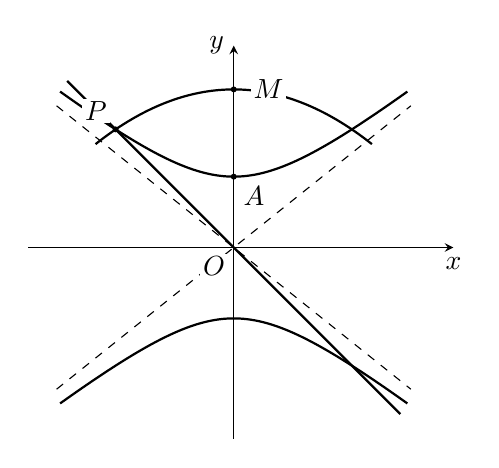
\begin{tikzpicture}[>=stealth,scale=0.9,line join=round]
  % 坐标轴
  \draw[->] (-2.9,0)--(3.1,0) node[below] {$x$};
  \draw[->] (0,-2.7)--(0,2.85) node[left] {$y$};
  % 渐近线 y=±0.8x
  \draw[dashed] (-2.5,-2.0)--(2.5,2.0);
  \draw[dashed] (-2.5,2.0)--(2.5,-2.0);
  % 双曲线 y^2 - x^2/1.5625 = 1
  \draw[thick,domain=-2.45:2.45,samples=90] plot (\x,{sqrt(1+\x*\x/1.5625)});
  \draw[thick,domain=-2.45:2.45,samples=90] plot (\x,{-sqrt(1+\x*\x/1.5625)});
  % 直线 y=-x
  \draw[thick] (-2.35,2.35)--(2.35,-2.35);
  % 抛物线 x^2 = -4.924(y-2.231)
  \draw[thick,domain=-1.95:1.95,samples=70] plot (\x,{2.231-0.2031*\x*\x});
  % 关键点
  \coordinate (P) at (-1.667,1.667);
  \coordinate (A) at (0,1);
  \coordinate (M) at (0,2.231);
  \fill (P) circle (1.2pt) node[fill=white,inner sep=1pt,above left=2pt] {$P$};
  \fill (A) circle (1.2pt) node[below right] {$A$};
  \fill (M) circle (1.2pt) node[fill=white,inner sep=1pt,right=6pt] {$M$};
  \node[fill=white,inner sep=1pt,below left=2pt] at (0,0) {$O$};
\end{tikzpicture}
\end{center}
\nopagebreak[4]
\Needspace{4\baselineskip}
\textbf{解析}

\Needspace{5\baselineskip}
由 $(1-a^{2})x^{2}+a^{2}y^{2}-a^{2}=0$ 是双曲线，知 $1-a^{2}<0$。两边除以 $a^{2}$ 并整理得

\nopagebreak[4]
\[
y^{2}-\frac{x^{2}}{\dfrac{a^{2}}{a^{2}-1}}=1.
\]

\Needspace{5\baselineskip}
故两条渐近线的斜率为 $\pm\dfrac{\sqrt{a^{2}-1}}{a}$。由条件

\nopagebreak[4]
\[
\frac{\sqrt{3}}{2}\le\frac{\sqrt{a^{2}-1}}{a}\le\frac{2\sqrt{2}}{3},
\]

\Needspace{5\baselineskip}
平方得 $\dfrac{3}{4}\le 1-\dfrac{1}{a^{2}}\le\dfrac{8}{9}$，即 $\dfrac{1}{9}\le\dfrac{1}{a^{2}}\le\dfrac{1}{4}$，故

\nopagebreak[4]
\[
4\le a^{2}\le 9,\qquad 2\le a\le 3.
\]

\Needspace{5\baselineskip}
将 $y=-x$ 代入双曲线方程，得 $(1-a^{2})x^{2}+a^{2}x^{2}-a^{2}=0$，即 $x^{2}=a^{2}$，故 $x=\pm a$。按图，$P$ 取第二象限的交点

\nopagebreak[4]
\[
P(-a,a).
\]

\Needspace{5\baselineskip}
上半支顶点为 $A(0,1)$。以 $A$ 为焦点、$M(0,m)$ 为顶点的开口向下的抛物线为

\nopagebreak[4]
\[
x^{2}=-4(m-1)(y-m).
\]

\Needspace{5\baselineskip}
因 $P(-a,a)$ 在其上，

\nopagebreak[4]
\[
a^{2}=-4(m-1)(a-m)=4(m-1)(m-a). \tag{①}
\]

\Needspace{5\baselineskip}
展开整理得

\nopagebreak[4]
\[
m^{2}-(1+a)m+\left(a-\frac{a^{2}}{4}\right)=0,
\]

\Needspace{5\baselineskip}
解得

\nopagebreak[4]
\[
m=\frac{1}{2}\left(1+a\pm\sqrt{1-2a+2a^{2}}\right).
\]

\Needspace{5\baselineskip}
由题设抛物线开口向下、顶点 $M(0,m)$ 在焦点 $A(0,1)$ 上方，知 $m>1$；又 ① 式右端为 $a^{2}>0$，故 $m-a>0$，即 $m>a$。于是 $m>\dfrac{1+a}{2}$，取加号：

\nopagebreak[4]
\[
m=\frac{1}{2}\left(1+a+\sqrt{1-2a+2a^{2}}\right).
\]

\Needspace{5\baselineskip}
直线 $PM$ 的斜率为

\nopagebreak[4]
\[
k=\frac{m-a}{0-(-a)}=\frac{m-a}{a}
=\frac{1}{2a}\left(1-a+\sqrt{1-2a+2a^{2}}\right).
\]

\Needspace{5\baselineskip}
令 $u=\dfrac{1}{a}$，由 $2\le a\le 3$ 得 $u\in\left[\dfrac{1}{3},\dfrac{1}{2}\right]$，且

\nopagebreak[4]
\[
k=\frac{1}{2}\left(u-1+\sqrt{u^{2}-2u+2}\right)
=\frac{1}{2}\left[\sqrt{(1-u)^{2}+1}-(1-u)\right].
\]

\Needspace{5\baselineskip}
有理化得

\nopagebreak[4]
\[
k=\frac{1}{2}\cdot\frac{1}{\sqrt{(1-u)^{2}+1}+(1-u)}.
\]

\Needspace{5\baselineskip}
在 $\left[\dfrac{1}{3},\dfrac{1}{2}\right]$ 上，$u$ 递减而 $1-u$ 递增，故 $(1-u)^{2}+1$ 递增，分母递增，$k$ 递减。于是 $k$ 在 $a=2$（即 $u=\dfrac{1}{2}$）处取最大值：

\nopagebreak[4]
\[
k_{\max}=\frac{1}{2}\left[\sqrt{\left(\frac{1}{2}\right)^{2}+1}-\frac{1}{2}\right]
=\frac{1}{2}\left(\frac{\sqrt{5}}{2}-\frac{1}{2}\right)
=\frac{\sqrt{5}-1}{4}.
\]

\gkanswer{答案：$\dfrac{\sqrt{5}-1}{4}$。}

\end{answer}